\chapter{Data Understanding and Preparation}
\label{ch:capitolo1}

The dataset \textit{train.csv} contains 16431 titles of different forms of visual entertainment that have been rated on IMDb, 
an online database of information related to films, television series etc. 
Each record is described by 23 attributes, both numerical and non-numerical. 
% All the variables of the dataset are introduced and explained in Table 1.1 and Table 1.2.


% \section{Distribution of the variables and statistics}\label{sec:variable_distrib}
% This section will give an overview about the distribution of variables that has been carried on to understand patterns, 
% detect meaningful statistics and assess their relevance to the project. 

\section{Discrete attributes}
Table~\ref{tab:attributes} shows the discrete attributes of the dataset,
their types and a brief description of each attribute.
\begin{table}[h]
    \centering
    \begin{tabular}{|l|l|l|} % Using 'l' for left alignment of columns
        \hline
        \textbf{Attribute} & \textbf{Type} & \textbf{Description} \\ 
        \hline
        \texttt{originalTitle} & Categorical & Title in its original language \\  
        \hline
        \texttt{rating} & Ordinal & IMDB title rating class \\
        & & The range is from \texttt{(0,1]} to \texttt{(9,10]} \\ 
        \hline
        \texttt{titleType} & Categorical & The format of the title \\ 
        \hline
        \texttt{canHaveEpisodes} & Binary & Whether or not the title can have episodes \\ 
        & & \texttt{True}: can have episodes; \texttt{False}: cannot have episodes \\ 
        \hline
        \texttt{isRatable} & Binary & Whether or not the title can be rated by users \\ 
        & & \texttt{True}: it can be rated; \texttt{False}: cannot be rated \\ 
        \hline
        \texttt{isAdult} & Binary & Whether or not the title is for adults \\ 
        & & \texttt{0}: non-adult title; \texttt{1}: adult title \\ 
        \hline
        \texttt{countryOfOrigin} & List & The country(ies) where the title was produced \\ 
        \hline
        \texttt{genres} & List & The genre(s) associated with the title (3 at most) \\ 
        \hline
    \end{tabular}
    \caption{Description of discrete attributes}
    \label{tab:attributes}
\end{table}

\subsection{Discrete attributes analysis}
This paragraph provides an overview of the discrete attributes in the dataset, focusing on their distributions and statistics.\\
The following figure~\ref{fig:titleType_distrib} shows an histogram of \texttt{titleType}.
\begin{figure}[H]
    \centering
    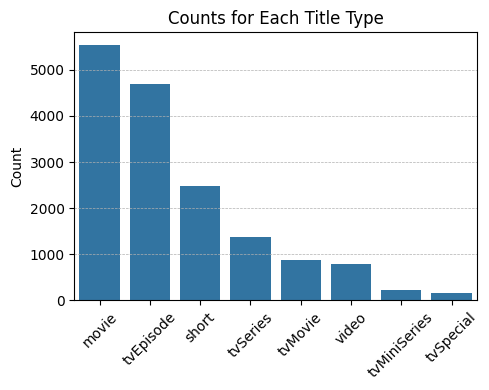
\includegraphics[width=0.65\textwidth]{plots/types_count.png}     %se teniamo 0.65 ci sta sotto la tabella delle continuous
    \caption{Distribution of the \texttt{titleType} attribute}
    \label{fig:titleType_distrib}
\end{figure}
It was observed that the class \textit{tvShort} is the least frequent in the dataset, with only 40 records (around 0.24\% of the dataset). Because of this, these rows were discarded from the dataset, as they were considered irrelevant for the analysis.
The decision was not repeated for \textit{tvSpecial} and \textit{tvMiniSeries}, as they cover slightly more than 1\% of the dataset each (166, 1.01\% and 224, 1.36\%, respectively).\\


% In this paragraph, the most informative discrete attributes of the dataset are examined to provide an overview of their statistics and frequencies. \\
% From figure~\ref{fig:sub1} it is observed that the classes of the \texttt{titleType} attribute are unbalanced, with \textit{movie} being 
% the most frequent class (5535 records) and \textit{tvShort} the least frequent (40 records). 
% By analyzing the \texttt{canHaveEpisodes} attribute within these \texttt{titleType} values, it is found that only \textit{tvSeries} and 
% \textit{tvMiniSeries} can have episodes, as expected.
% As shown in figure~\ref{fig:sub2}, the frequency of rating classes is slighly skewed toward higher values, with the most frequent rating 
% class being (7, 8], which is the rating of 4822 titles.
% Another important aspect is that all 16341 titles are ratable and the vast majority of them (16005) are non-adults contents, as shown 
% in figure~\ref{fig:sub3}
% Finally, as indicated in figure~\ref{fig:sub4}, an analysis of the \texttt{genres} variable across different \texttt{titleType} values 
% reveals that \textit{Drama} and \textit{Comedy} are the most common genres, as they appear in the top 3 genres of nearly every \texttt{titleType} category.


% \begin{figure}[H]
%     \centering
%     % First subfigure
%     \begin{subfigure}{0.48\textwidth}
%         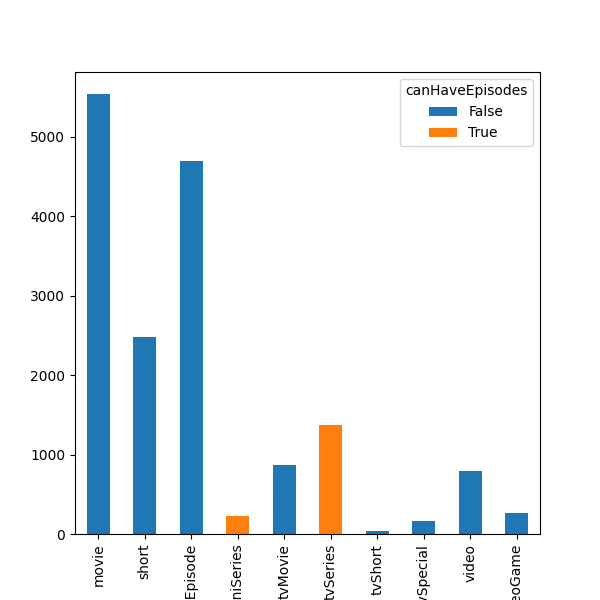
\includegraphics[width=\textwidth]{plots/fig1_a.png}
%         \caption{Counting of the title types frequencies} %  combined with the canHaveEpisodes variable
%         \label{fig:sub1}
%     \end{subfigure}
%     \hfill
%     % Second subfigure
%     \begin{subfigure}{0.48\textwidth}
%         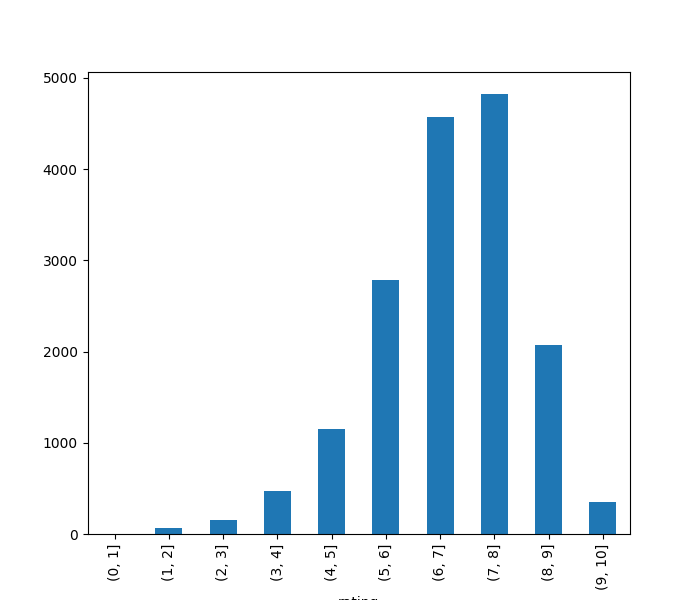
\includegraphics[width=\textwidth]{plots/fig1_b.png}
%         \caption{Counting of ratings frequencies}
%         \label{fig:sub2}
%     \end{subfigure}
    
%     % Third subfigure
%     \begin{subfigure}{0.48\textwidth}
%         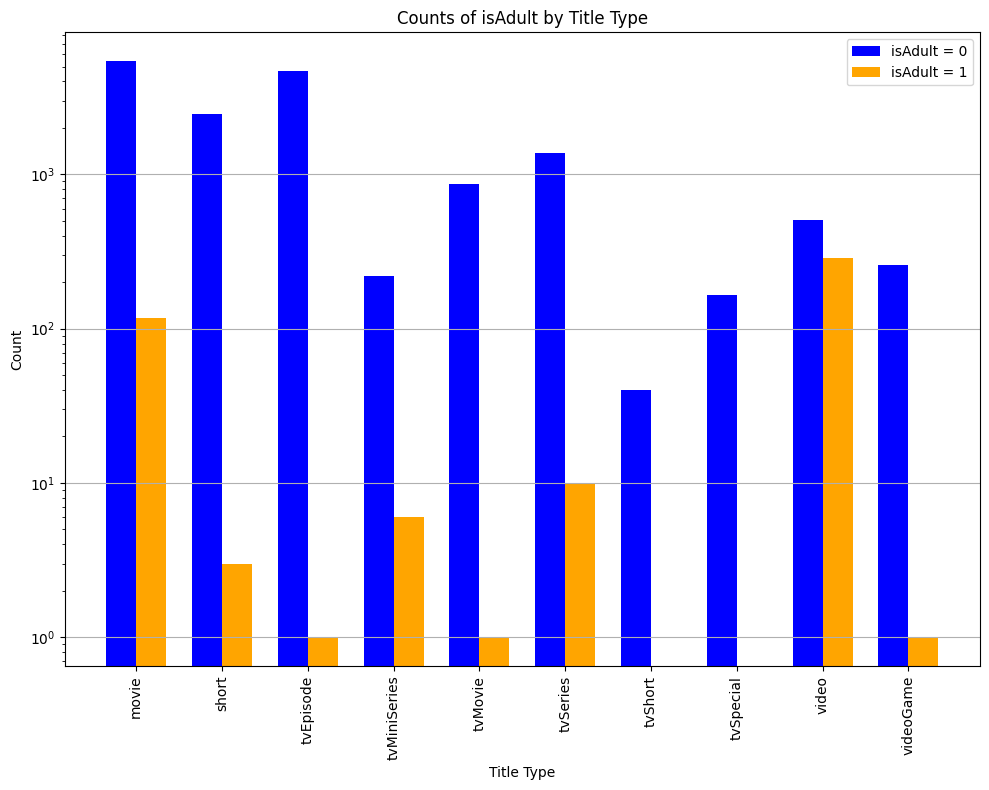
\includegraphics[width=\textwidth]{plots/fig1_c.png}
%         \caption{Counting of the adult and non-adult per type}
%         \label{fig:sub3}
%     \end{subfigure}
%     \hfill
%     % Fourth subfigure
%     \begin{subfigure}{0.48\textwidth}
%         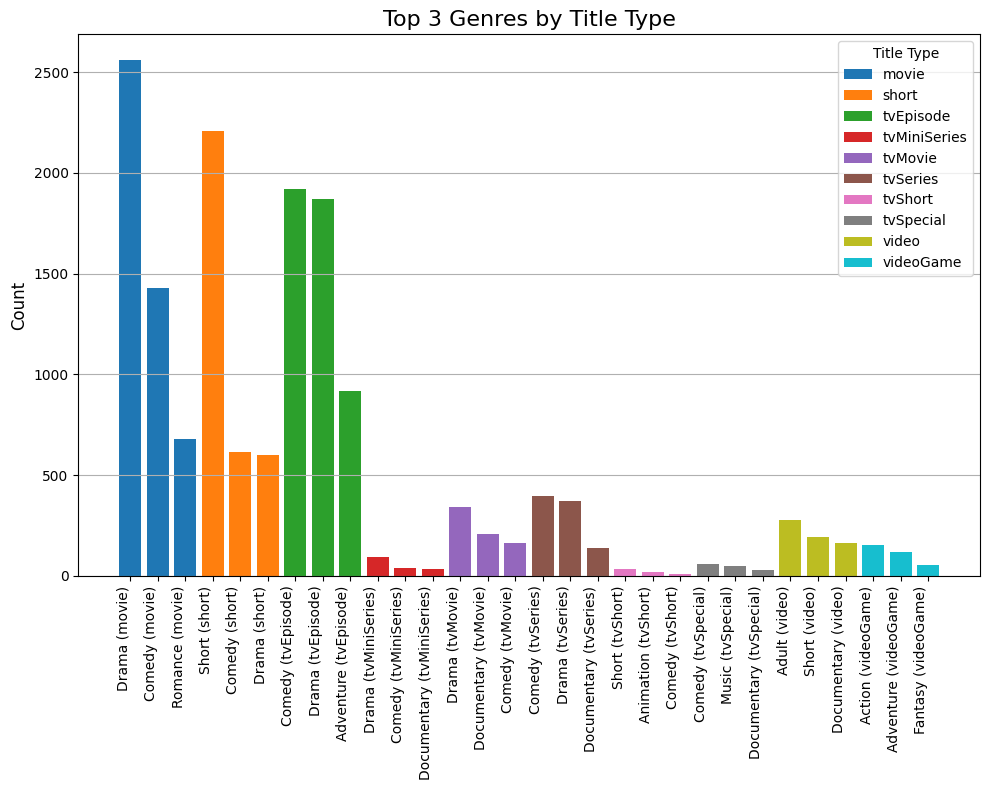
\includegraphics[width=\textwidth]{plots/fig1_d.png}
%         \caption{types per genre}
%         \label{fig:sub4}
%     \end{subfigure}
    
%     \caption{Bar chart of the discrete attributes.}
%     \label{fig:bar-charts}
% \end{figure}


\subsection{Merging and Removal of Categorical Attributes}\label{subsec:var_elim_discrete}
The following categorical attributes were removed from the dataset:
\begin{itemize}
    \item \texttt{originalTitle} was removed because it is not relevant for the analysis;
    \item the \texttt{isRatable} variable was removed because all the titles in the dataset are ratable;
    \item \texttt{worstRating} and \texttt{bestRating} attributes were removed because they assume the same values for all records (1 and 10 respectively).
\end{itemize}

Additionally, the \texttt{isAdult} attribute is highly correlated with the presence or absence of
\textit{Adult} in \texttt{genre} (16 records differ in the train set, 1 in the test set), so the two were
merged with a logical OR operation.


\subsection{Encoding and Transformation of Categorical Attributes}
% \texttt{countryOfOrigin} and \texttt{genres} variables (datatypes: strings) were converted into 
% lists of strings to facilitate further analysis.
% This transformation was necessary because some records contain multiple genres or countries as values for
% these variables.
The attribute \texttt{rating} was converted into an ordinal variable by taking the upper bound of each rating
interval's string representation. This approach was chosen because the minimum rating is 1, meaning the
lowest interval corresponds only to ratings of 1. For consistency, the same transformation was applied
to all other intervals.\\

Multi-label one-hot encoding was applied to the \texttt{genres} column. 
Each unique genre was represented as a binary feature, allowing records that belong to multiple genres simultaneously to maintain this information; this generated 28 new attributes.
Rows with no genres were assigned a vector of all zeros, indicating the absence of any genres.\\

% After that, multi-label one-hot encoding was applied to the
% \texttt{genres} column; each unique genre was represented as a binary feature, 
% allowing records that belong to multiple genres simultaneously to maintain this information.
The attribute \texttt{countryOfOrigin} was represented by grouping the countries by continent.
The following variables have been created: 
\begin{multicols}{2}
    \begin{itemize}
        \item \texttt{countryOfOrigin\_AF} (Africa);
        \item \texttt{countryOfOrigin\_AS} (Asia);
        \item \texttt{countryOfOrigin\_EU} (Europe);
        \item \texttt{countryOfOrigin\_NA} (North America);
        \item \texttt{countryOfOrigin\_SA} (South America);
        \item \texttt{countryOfOrigin\_OC} (Oceania);
        \item \texttt{countryOfOrigin\_UNK} (Unknown country);
        \item \texttt{countryOfOrigin\_freq\_enc} (frequency encoding of the original list).
    \end{itemize}
\end{multicols}

Each of the first six features provides the number of countries in the corresponding continent.
\texttt{countryOfOrigin\_UNK} is used to represent the strings that are not categorized as being part of a
continent, by again counting the strings that are not recognized.
The feature \texttt{countryOfOrigin\_freq\_enc} provides the frequency encoding of the
original list as a whole.
In summary, the original attribute is represented by the seven features regarding
the continents, plus 1 representing the frequency encoding. This representation was chosen as it allows to
keep a lot of the original information, while limiting the number of new features.\\




\section{Continuous Attributes}
Table~\ref{tab:numerical_attributes} shows the continuous attributes of the dataset,
a brief description as well as their type.
\begin{table}[h]
    \centering             
    
    %nel type secondo me ha senso mettere il tipo di variabile continua (quindi interval, ratio ecc.)        

    \begin{tabular}{|l|l|l|} 
        \hline
        \textbf{Attribute} & \textbf{Type} & \textbf{Description} \\
        \hline
        \texttt{worstRating} & Float & Worst title rating \\ 
        \hline
        \texttt{bestRating} & Float & Best title rating \\ 
        \hline
        \texttt{runtimeMinutes} & Integer & Runtime of the title expressed in minutes \\ 
        \hline
        \texttt{startYear} & Integer & Release/start year of a title \\ 
        \hline
        \texttt{endYear} & Integer & TV Series end year \\
        \hline
        \texttt{awardWins} & Integer & Number of awards the title won \\ 
        \hline
        \texttt{numVotes} & Integer & Number of votes the title has received \\ 
        \hline
        \texttt{totalImages} & Integer & Number of Images on the IMDb title page \\ 
        \hline
        \texttt{totalVideos} & Integer & Number of Videos on the IMDb title page \\ 
        \hline
        \texttt{totalCredits} & Integer & Number of Credits for the title \\ 
        \hline
        \texttt{criticReviewsTotal} & Integer & Total Number of Critic Reviews \\ 
        \hline
        \texttt{awardNominationsExcludeWins} & Integer & Number of award nominations excluding wins \\ 
        \hline
        \texttt{numRegions} & Integer & The regions number for this version of the title \\ 
        \hline
        \texttt{userReviewsTotal} & Integer & Number of User Reviews \\ 
        \hline
        \texttt{ratingCount} & Integer & The total number of user ratings for the title \\ 
        \hline
    \end{tabular}
    \caption{Description of continuous attributes}
    \label{tab:numerical_attributes}
\end{table}


\subsection{Removal and Merging of Continuous Attributes}\label{sec:var_elim_creation}
% The \texttt{worstRating} and \texttt{bestRating} attributes were removed from the dataset because they
% assume the same values for all records of the dataset (1 and 10 respectively).\\
%                       questi li ho messi in 1.1.2 dato che sono ordinal anche loro mi sa

The plot in figure~\ref{fig:correlation_matrix} is a Pearson's correlation matrix that takes into
account the continuous attributes of the dataset.\\

\begin{figure}[H]
    \centering
    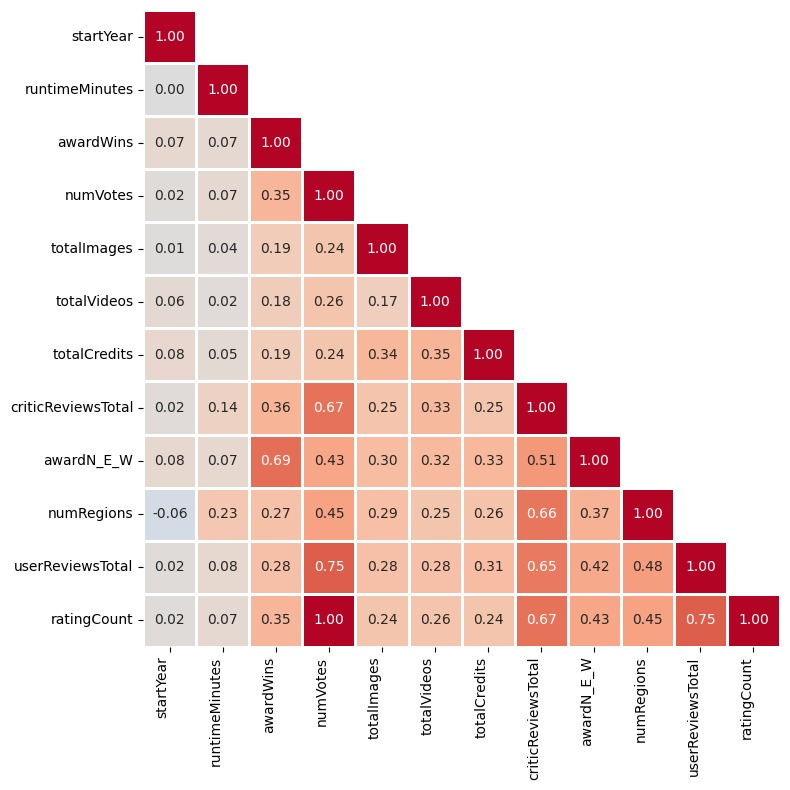
\includegraphics[width=0.65\textwidth]{plots/correlation_matrix.png}
    \caption{Correlation matrix of the numerical features}
    \label{fig:correlation_matrix}
\end{figure}


The correlation matrix shows that \texttt{ratingCount} and \texttt{numVotes} are perfectly correlated;
for their redundancy, \texttt{ratingCount} was discarded.\\

The two attributes \texttt{awardWins} and \texttt{awardNominationsExcludeWins} were combined into a single
feature, i.e. \texttt{totalNominations}, due to their strong semantic similarity and high correlation (0.95).
The new feature represents the sum of the two original attributes. This transformation also helps
mitigate the impact of their heavy left skew (shown in figure \ref{fig:sub1}), resulting in a more meaningful and interpretable feature.\\

Similarly, the \texttt{totalVideos} and \texttt{totalImages} attributes were combined into a single
feature, i.e. \texttt{totalMedia}, representing the total number of media items associated with a title.
Although the original attributes are not highly correlated, both exhibit skewed distributions (as shown in figure \ref{fig:sub2}), the first in particular.
Due to this, and their similar semantic meaning, they were merged to form a more consolidated and
interpretable feature.

\begin{figure}[H]
    \centering
    % First subfigure
    \begin{subfigure}{0.48\textwidth}
        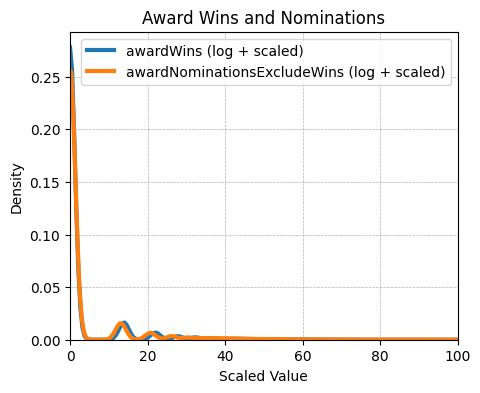
\includegraphics[width=\textwidth]{plots/nominations_distrib.png}
        \caption{Logarithmic distribution of the \texttt{totalNominations} attribute}
        \label{fig:sub1}
    \end{subfigure}
    \begin{subfigure}{0.48\textwidth}
        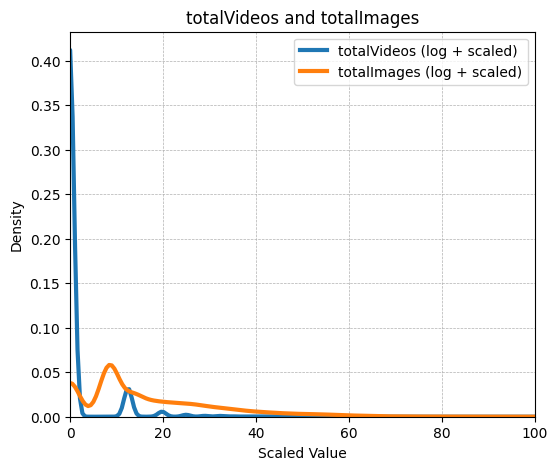
\includegraphics[width=\textwidth]{plots/totalVideos_Images_distrib.png}
        \caption{Logarithmic distribution of the \texttt{totalNominations} attribute}
        \label{fig:sub2}
    \end{subfigure}
    \caption{Distribution of the \texttt{totalNominations} and \texttt{totalMedia} attributes}
    \label{fig:distrib}
\end{figure}



\section{Data Quality}\label{sec:data_quality}
Next, a proper evaluation of the observed data was conducted in preparation for the analysis.
Once having checked that there are no duplicates and no incomplete rows in the dataset, 
attention was given at identifying missing values and outliers.



% \subsection{Syntactic Inconsistencies}
% In the exploration of the dataset it has been noticed that \texttt{awardWins} was the only feature having missing values marked with \texttt{NaN}.
% However, there were missing values also in other columns (\texttt{endYear}, \texttt{runtimeMinutes} and \texttt{genres}), 
% but they were indicated with the string "\textbackslash N".
% To avoid this inconsistency that might have caused problems during data preparation, these values have been replaced with \texttt{NaN}.
% By doing so, any cell in the \texttt{endYear}, \texttt{runtimeMinutes} and \texttt{genres} columns 
% that previously contained the string "\textbackslash N" is now considered a proper missing value, detectable and manageable using Pandas' functions.



\subsection{Missing Values}
% Once having solved the above-mentioned inconsistency, the resulting total amount of the missing values are the following, 
% also represented in percentages for a better understanding:
After the previously mentioned changes, the dataset was checked for missing values.
These attributes were found to have missing values:
\begin{itemize}
    \item \texttt{endYear}: it is the feature with the highest number of NaN values (15617; about 95\%).
    Although the feature is only relevant for \textit{TVSeries} and \textit{TVMiniSeries} titles, it still
    had approximately 50\% missing values within those categories, limiting its usefulness even in the
    appropriate context. For this reason, the feature was discarded.
    
    \item \texttt{runtimeMinutes}: this attribute has 4,852 missing values (29.5\%). Two imputation strategies were employed, both based on random sampling within the interquartile range. 
    One strategy used the \texttt{titleType} feature to define the range, while the other imputed values independently of any other features. 
    The choice of which of the two strategies to use depends on the specific task, and will be specified in the corresponding sections.
    % by grouping the records by \texttt{titleType} and substituting the NaN value with the median of each group \textbf{ALTRIMENTI prendere valore random tra il 30\% - 70\% per titletype; anche se questo causa problemi nel momento in cui andiamo a classificare un nuovo record che non ha titletype};
    
    \item \texttt{awardWins}: this feature has 2618 NaN values (about 16\%).
    Since the mode associated with this variable is 0, it has been decided to substitute the missing
    values with 0.

    \item \texttt{genres}: it has 382 missing values (2.3\%). Having dealt this variable with a
    multi-label one-hot encoding process (as will be described in the \textit{Variable Transformation}
    section), a vector of all zeros is assigned to record with missing genres values.
\end{itemize}



\subsection{Semantic Inconsistencies, Outlier detection and Feature Transformations}
While analyzing the dataset, it was observed that the \textit{Videogame} type of the \texttt{titleType} attribute (which consists of 259
records - around 1.58\% of the dataset) was not consistent with the other attributes. 
Other then the semantic inconsistency, these rows
generated problems for some of the other attributes, such as \texttt{runtimeMinutes}, resulting in most
values being missing (and difficult to impute). Because of this problem, as well as the meaning discrepancy, the samples were removed from the dataset because it was deemed to be semantically inconsistent with the other title types.\\
% While examining the dataset, it became apparent that some attributes have outliers. 
% The important aspect to highlight is that since \texttt{awardWins}, \texttt{totalVideos} 
% and \texttt{awardNominationsExcludeWins} have many values as 0 (respectively 11971, 14821, 14427), 
% these might be considered variables with many outliers 
% (as seen in Figure \textbf{METTERE GRAFICO che rappresenti in qualche modo il result di DETECT\_OULIERS\_MULTI\_ATTRIBUTES in data\_quality noemi}) 
% but they actually have less outliers compared to the other variables.
% For the other attributes \textbf{CONTINUARE......}
% \textbf{VALORI OUTLIERS SU TRAIN IN \%: 86.7 , 90.2 , 87.8}
% \textbf{VALORI OUTLIERS SU DF\_PP IN \%: 88.7 , 90.2 , 87.8}


% As for the continuous attributes, it was observed that they required a stronger transformation due to their highly positively skewed distributions. 
% Specifically, when required by the data mining method, a log-transformation was applied to all the numeric attributes, since their skewness was highly greater than 1. 
% Following the log-transformation, standard normalization techniques - \texttt{MinMaxScaler} and \texttt{StandardScaler} - have then been applied (when scaling was necessary); 
% respectively to scale each feature to a given range and to standardize features by removing the mean and scaling to unit variance.
% The decision to apply one or the other was again made based on the specific requirements of each data mining technique, and so will be specified accordingly in each section.
% \textbf{CONTROLLARE SE IN OGNI SEZIONE C'E' SPECIFICA SULLE DUE NORMALIZZAZIONI USATE!!!}.


